\section{Humans may be Everywhere}

Here are some topics that I've been exploring, when the \emph{Masked Singer} was not available. Some will become full essays, some not.

\paragraph{Vanity}
All is vanity. Everyone on social media is promoting the next book, the next translation, youtube video, or seeking new followers and new ``likes". But for what purpose? All is vanity.

\begin{wrapfigure}{rt}{.3\textwidth}
 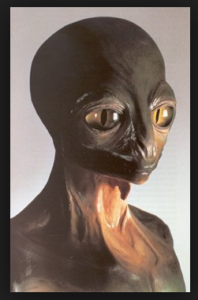
\includegraphics[scale=.5]{a20211124HumansMayBeEverywhere-img001.png}
\end{wrapfigure}

\paragraph{Metaphysics and Physics}
Reality has an inside and an outside. Metaphysics, as the study of being, is concerned with the inside, and physics that of becoming and the outside. Hence, metaphysics is constant while physics changes. As such, metaphysics is certain and absolute, so it cannot be regarded as a ``philosophical system" in the contemporary understanding of the term.

The phrase, the transcendental unity of religion, is somewhat misguided, since it fails to recognize the unmistakable differences in religions. What is correct is that the higher traditions share and understand the same metaphysics. The metaphysic is the genus and the species is the exoteric religion.

\paragraph{Evolution and Wings}
Darwinian evolution cannot explain, if mutations are random, why and how evolution progresses from simple to complex life forms. Pumpkin Person ponders why Evolution is progressive\footnote{\url{https://pumpkinperson.com/2021/02/14/evolution-is-progressive-debunking-goulds-drunkard-walk-metaphor/}}.

Scientists Say There May Be ``Humans" All Over the Universe: Humans are Everywhere\footnote{\url{https://futurism.com/scientists-humans-universe}}

The new theory is that evolution is not quite random, but rather that it converges to predictable forms. For example, the wing evolved independently in birds, bats, insects and pterosaurs. That makes no sense unless we presume there is a prototype of a wing that manifests itself in different creatures. Valentin Tomberg explains this based on traditional sources that predate ``science" by millennia:

\begin{quotex}
Tentacles, paws, arms, wings —are they not simply diverse forms manifesting a common prototype or principle? They are in so far as they express the desire to bear the sense of touch further, to be able to touch things more removed than those in the immediate neighbourhood of the surface of the body.

The organs of action are simply crystallised will. The ``what" of the will engenders the ``how" of the action (the organ), and not inversely. It is similar with wings. They are also an exteriorised will — a will become organ. This is the will to go out from the usual orbit not only in the horizontal but also in the vertical, not only to bear touch forward, but also to bear it above. Wings express the will for movement according to a cross, i.e. not only that of expansion on a plane but also that of elevation to another plane.

\end{quotex}
\paragraph{End time prophecy}

\textbf{Hildegard of Bingen} was a Saint and Doctor of the Church from nearly 1000 years ago. In her masterwork \emph{Scivias} she uses the symbolism of five beasts to explain the stages of the end times: the red dog, the yellow lion, the pale horse, the black pig, and the grey wolf. If you are an animal lover, or just would like to know what to expect next, the blog \textit{The Five Beasts}\footnote{\url{https://thefivebeasts.wordpress.com/the-five-beasts-in-a-nutshell/}} attempts to relate Hildegard's vision to our own times. Regarding the final stage of the Grey Wolf, she writes:

\begin{wrapfigure}{rt}{.3\textwidth}
 
\includegraphics[scale=2]{a20211124HumansMayBeEverywhere-img002.jpg} 
 \caption{Grey Wolf}
\end{wrapfigure} 

\begin{quotex}
It is interesting that Hildegard goes into far more detail regarding the Grey Wolf than the other eras. Essentially, three main things will define the era:

\begin{itemize}
\item Civil unrest and revolutions with their cause being economic inequality. 
\item Physical persecution of the Church by a specific group of people. 
\item A powerful spiritual revival in the Church. 
\end{itemize}

She also adds that it is when the Church will be ``…replete with the full number of her children." The Church's mission to evangelize will have been completed.

\end{quotex}
\paragraph{Satan's revelation}
I don't think it is wise to believe anything that Satan says. But if you do, you might be interested in this discussion: Exorcist says Satan's Time is running short\footnote{\url{https://www.lifesitenews.com/news/exorcist-says-satans-time-is-running-short/}}.

\paragraph{Signs of the End of Time}
Here is a Muslim perspective on the end of times\footnote{\url{https://www.youtube.com/watch?v=hyHv6Mx0oJ0}}, which tracks Rene Guenon more or less closely.

\begin{itemize}
\item Prophecy of Phones 
\item Prophecy of the Talking Shoe 
\item Inanimate Objects would speak 
\item Rulers are the lowest people 
\item No people are left except the dregs 
\item Entertainers, prostitutes — the lowest of people — will be the happiest 
\item The far will become near 
\end{itemize}
\paragraph{Four horsemen of meaning}
Jordan Peterson created a fictitious group calling itself the ``Dark Enlightenment". It fractured as one of them was deplatformed and probably no one really got enlightened. Undeterred, Peterson has created a new group calling itself the Four Horsemen of Meaning, including himself and three others he recruited.

It seems to me that the symbol of the Four Horsemen is the worst possible one to use, as it calls to mind the Four Horsemen of the Apocalypse. I suppose this is fine for men and women who are unable to find meaning in their lives, so they need it regurgitated like a mama bird feeding her brood.

Unfortunately, this is an impossible task. Meaning is never found independently in the object, but only in relation to a Self. Hence, Meaning cannot be inserted into the mind; rather it the Self expresses its meaning through its acts. See this essay on Hermann Keyserling\footnote{\url{https://www.gornahoor.net/?p=7437}} for how to think about meaning.

\paragraph{IQ and ignorance}
The topic if intelligence, IQ, and their relationship will be explored soon. So I did a field study of some really high IQ people. Since it is impossible to sustain a serious discussion on social media because not everyone is equal, I thought I would try one devoted to those with IQs in the 99.9 percentile (one in a thousand).

I posted a short video about Schopenhauer, who certainly had a high IQ, whatever your opinion might be of his philosophy. See \textit{Why Smart People Don't Care About Being Social}\footnote{\url{https://www.youtube.com/watch?v=_oR78_QVF8s}}.

I thought it would be appropriate to that group. One fellow ranted about it, proclaiming that Tolstoy's ethical views were superior to Schopenhauer's. I gently pointed out that Tolstoy was deeply influenced by Schopenhauer, as documented in Leo Tolstoy: Religious and political beliefs\footnote{\url{https://en.wikipedia.org/wiki/Leo_Tolstoy\#Religious_and_political_beliefs}}.

The ability to solve puzzles and find patterns does is not the same as understanding the deep meanings of things.

\paragraph{Inanities}
Social media is replete with inanities that are regarded as highly motivational and deeply spiritual. But there is nothing in them about bearing wrongs patiently, submission to the will of God, self-knowledge, purification of the mind and will, or the pursuit of a virtuous life.

\paragraph{Neuroscience and free will}
A neuroscientist debunks ``free will" because he sees some electrical activity in the brain as the subject is making a decision. That means that these weird neurons know in advance whether I will choose pistachio or chocolate gelato while I am on the way to the gelateria. The moderator chooses not to pursue this line of questioning in \textit{Patrick Haggard — Is Free Will an Illusion?}\footnote{\url{https://www.youtube.com/watch?v=lKKZdzVbIOs}}

I just found this\footnote{\url{https://mindmatters.ai/2021/11/does-science-disprove-free-will-a-physicist-says-no/}} today that debunks that very experiment.

\flrightit{Posted on 2021-11-24 by Cologero }

\begin{center}* * *\end{center}

\begin{footnotesize}\begin{sffamily}



\texttt{Cologero on 2021-12-15 at 06:31 said: }

The idea of humanoid creatures descended from dinosaurs has been part of the human collective unconscious, and has been part of folklore. Consider, for example:

\begin{quotex}
Edgar Rice Burroughs' Pellucidar series featured primitive dinosaur-descended humanoids living in the Hollow Earth called the Horibs or snake-men in his 1929–1930 crossover Tarzan at the Earth's Core.

\end{quotex}
Source Reptilian Humanoid

This fits into today's UFO speculation about their source being the hollow earth. The point is that the possibility of reptilian humanoids may actually be a plausible idea. This post is intended to be a thought experiment for people with an imagination. It is off the mark to interpret it as a debate about Darwinism or as an assertion that such beings actually exist.


\hfill

\texttt{Balder on 2021-12-19 at 13:32 said: }

Wolfgang Smith believes that the answer to the problem of free will is in what he calls Vertical Causation (in Physics and Vertical Causation), namely that humans who possess a rational soul have access to the equivalent of a Cosmogenic Act. Sounds plausible to me even if free will exists only as a potential.


\end{sffamily}\end{footnotesize}
